

\chapter{Testování a~evaluace}


V této kapitole popisujeme, jak je celá aplikace otestována. Dále pak porovnání odhadů zpoždění se stávajícím řešení.

\bigbreak

Dosažené výsledky demonstrujeme v řadě případů na grafech. Tyto grafy byly vytvořeny pomocí knihovny jazyka Python 3 matplotlib a zdrojový kód je napsán ve složce TODO.

\section{Testování softwarového řešení}

Kód práce popsaný v~kapitole \ref{chapter:implementace} je otestován unit testy. Propojení tohoto softwaru s~databází i~zdrojem vstupních dat je testováno integračními testy.


\subsection{Unit testy}

Unit testy testují správnou funkčnost jednotlivých metod všech softwarových komponentů této práce.

\bigbreak

Pro ověření správné funkčnosti některých metod jsou vygenerována vstupní či výstupní data. To je z~důvodu, že tyto metody pracují s~komplexní datovou strukturou nebo s~velkým objemem dat, který není možno zadat jako vstup přímo v~kódu testu, resp. je potřeba porovnat výstup testované metody a~ze stejných důvodů není možné uvádět výstupní hodnoty pro porovnání přímo v~kódu testu. Typickým příkladem takové vstupní struktury je model profilu jízdy, protože je potřeba otestovat funkce, které s~takovým modelem pracují.

\bigbreak

Unit testy jsou k~nalezení v~příloze ve složce tests/unit.


\subsection{Integrační testy}

Integrační testy testují propojení jednotlivých modulů. Dále také testujeme správnou funkčnost databáze a~její funkce.

\bigbreak

Dále se testuje i~kompletní běh aplikace, kde se využívají stažená data.

\bigbreak

Integrční testy jsou dostupné v~příloze ve složce tests/integration


\subsection{Testy kvality}


Všechny následující výkonnostní testy jsou prováděny na osobním notebooku s~technickými parametry uvedenými v~tabulce \ref{table:hw}\footnote{https://9to5mac.com/2016/11/01/the-late-2016-entry-level-13-macbook-pro-has-a-ridiculously-fast-ssd/}.


\begin{center}
   \begin{table}[ht]
\centering
\begin{tabular}{|c|c|}
\hline
Parametr & Hodnota \\ \hline \hline
Procesor & 4x Intel(R) Core(TM) i7 CPU @ 2.70 GHz\\ \hline
Paměť & 16 GB DDR3 RAM  \\  \hline
Rychlost zápisu na disk & 1000--3000 MB/Sec \\ \hline
OS & macOS Big Sur\\ \hline
MySQL & version 8.0.18\\ \hline
\end{tabular}
\label{table:hw}
\end{table}
\end{center}


\bigbreak

Pro potlačení zkreslení testů vlivem čekání na stažení dat z~internetu jsou všechna data načítána z~disku počítače.


\bigbreak

Testování stejně jako funkční a~kvalitativní požadavky na práci vychází z~analýzy vstupních dat uvedené v~kapitole \ref{subsubsection:vstupni_soubory}.


\subsubsection{Zpracování dat}

Zpracování dat probíhá přečtením souboru s~polohy vozidel a~dále zpracovává každé vozidlo zvlášť. Přičemž pokud je vozidlo již nalezeno a~jeho poloha se od poslední aktualizace změnila, provedou se pouze dvě čtení z~databáze. Jeden záznam se aktualizuje a~vloží se jeden nový záznam\footnote{ověření existence spoje v~tabulce trips, načtení jízdního řádu z~tabulky rides, aktualizace dat spoje v~tabulce trips a~vložení aktuální polohy vozidla do tabulky skladující historická data \texttt{trip\_coordinates}}. Pokud je vozidlo již nalezeno a~jeho poloha se od poslední aktualizace nezměnila, provede se pouze jedno čtení z~databáze. Pokud ovšem je vozidlo obsluhující spoj nenalezeno, musí se číst soubor s~detailem daného spoje a~všechna data se vkládají do databáze (jízdní řád včetně zastávek), navíc geografická lomená čára popisující jízdu se ukládá jako soubor.


\bigbreak

Jak je ale vidět na grafu \ref{fig:file_process_time} i~pro nejvyšší množství vozidel (720) celé zpracování trvá nanejvýš 1,2 sekundy. Z~toho plyne, že samotné zpracování dat není nijak časově náročné a~vzhledem k~20sekundové periodě aktualizace dat máme velkou časovou rezervu. Rychlost zpracování jednoho vstupního souboru může více ovlivnit stahování dat z~internetu, kde ale předpokládáme, že po většinu času nebude trvat stáhnout aktuální polohy vozidel déle než desítky milisekund.

\begin{figure}
   \centering
 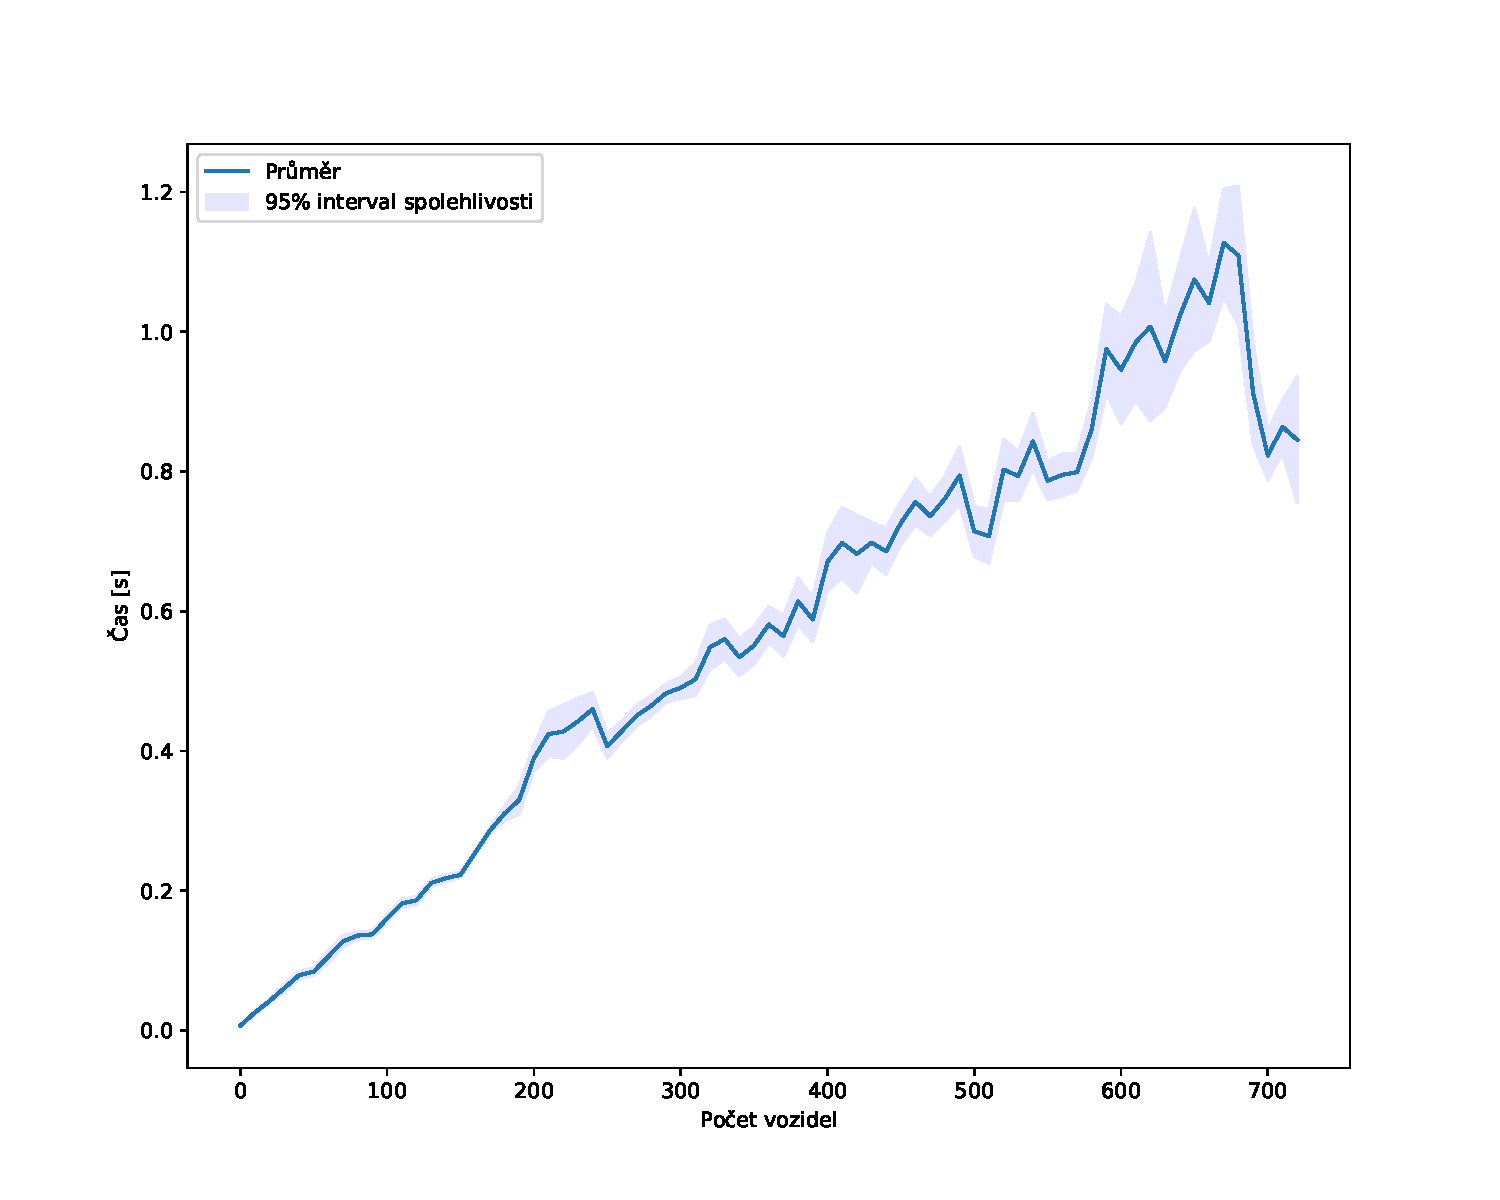
\includegraphics[width=\linewidth]{../img/file_process_time}
 \caption{Průměrný čas zpracovávání daného počtu vozidel ze všech souborů se statickými daty s~95\,\% intervalem spolehlivosti. Počty vozidel jsou vždy zaokrouhleny dolů na celé desítky.}
 \label{fig:file_process_time}
\end{figure}


\bigbreak

Jediné delší prodlení může nastat ve chvíli, kdy je potřeba stáhnout velké množství dodatečných informací o~novém spoji. Na grafu \ref{fig:vehicle_pos_x_new_trips} je vidět, že až na jednotky výjimek je počet nově nalezených spojů v~jednom souboru nejvýše 20. Aplikace je ale naimplementována tak, aby se tyto informace stahovaly asynchronně, a~tedy čekání na stažení dat bylo co nejkratší.


\subsubsection{Konstrukce modelů}

Po využití testovacích dat vzorků poloh vozidel zaznamenaných ve dnech 20.--24.\,2.\,2020 bylo podle kritérií, kterými jsou zejména vzdálenost zastávek a~počet vzorků mezi nimi, sestrojeno celkem 1\,106 polynomiálních modelů. Z~toho je 847 modelů pro pracovní dny, které jsou nejdůležitější. Přičemž celkový počet párů zastávek je 7\,230, ale zastávek ve vzdálenosti 1\,500 metrů\footnote{zvolená minimální vzdálenost mezi zastávkami, mezi kterými má ještě smysl odhadovat zpoždění} je pouze 2\,142. Z~toho vychází, že u~40\,\% dvojic zastávek je dostatek dat, aby dával výpočet modelu smysl.

\bigbreak

U zbylých dvojic zastávek se využívá lineární model.


\bigbreak

Čtení dat potřebných pro trénování modelů z~databáze, kde jsou data ze 4 dnů, trvá přibližně 110 sekund. Čtení se totiž provádí komplikovaným \gls{sql} dotazem uvedeným v~kapitole \ref{subsection:cteni_dat}, ovšem na rychlost provedení tohoto dotazu i~konstrukce modelů celkem neklademe žádné časové nároky, protože přepočítávání modelů je plánováno na čas nejmenšího zatížení systému, což bývá typicky v~noci.

\bigbreak

Dále ověřme, že výsledek dotazu nezahltí paměť počítače. Dotaz sice umožňuje čtení dat po stránkách, ale v~implementaci se tato vlastnost nevyužívá. Určení velikosti objektu jazyka Python 3 v~paměti počítače není úplně triviální úloha, protože v~paměti není objekt uložen na jednom místě, na části objektu se totiž ukazuje pointery\footnote{https://docs.python.org/3/reference/datamodel.html\#objects-values-and-types}. Dobrý odhad nám, ale poskytne uložit objekt na disk pomocí knihovny \verb-pickle-\footnote{https://docs.python.org/3/library/pickle.html}. Takto uložený objekt zabírá necelých 10\,MB prostoru na disku.


\bigbreak

Samotné zpracování dat a~trénování modelů trvá pro všech 2\,142 párů zastávek přes 2~minuty. Pro jeden pár zastávek je průměrná doba běhu 57 milisekund. Nejdéle trvá výpočet modelů 1,2 sekundy, a~to v~případě, kdy se zpracovává dohromady přes 10\,000 vzorků poloh vozidel.


\subsubsection{Serverová část uživatelské aplikace}

Server odpovídá na všechny typy požadovaných dotazů.

\bigbreak

Server je schopný odbavit přinejmenším 100 dotazů za sekundu. Na grafu \ref{fig:server_response_time} je zobrazeno jako dlouho trvalo serveru odpovědět na 100 paralelních dotazů, celkem v~1\,000 případech. Průměrná odpověď trvala třetinu sekundy a~jen v~jednom případě jsme na odpověď čekali 0,8 sekundy, tedy stále ještě pod jednu sekundu.

\begin{figure}
   \centering
 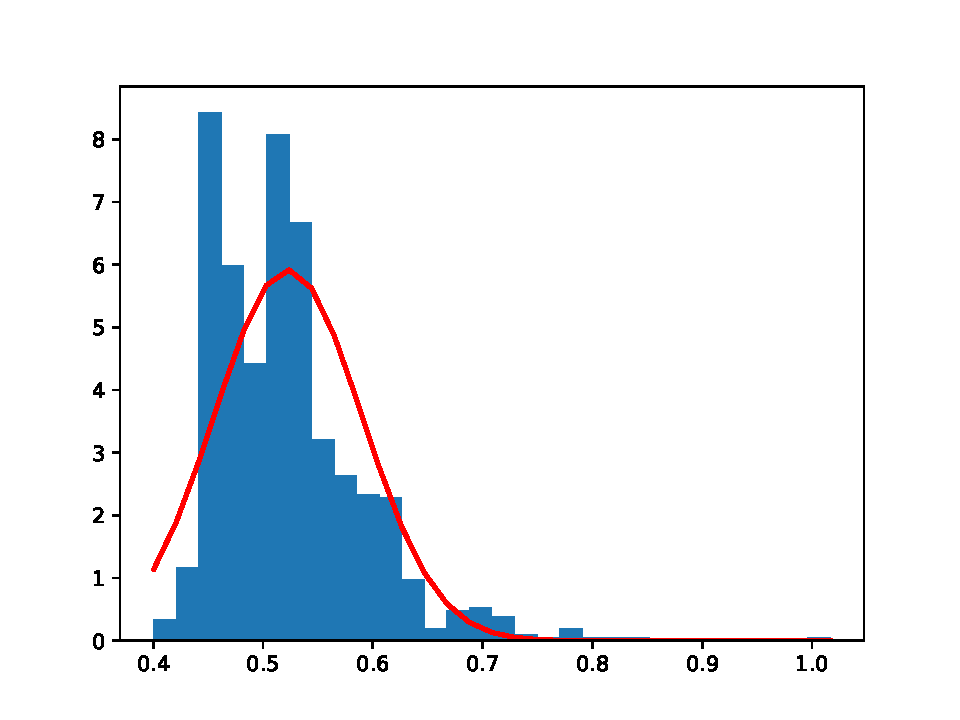
\includegraphics[width=\linewidth]{../img/server_response_time}
 \caption{Doba odpovědi serveru na 100 paralelních dotazů (1000 vzorků)}
 \label{fig:server_response_time}
\end{figure}


\subsubsection{Vizualizace}

Zátěžové testování vizualizační aplikace se dělá poměrně obtížně. Prakticky je pro testování jakékoliv front-endové aplikace vždy potřeba spustit aplikaci na konkrétním zařízení a~pozorovat její chování a~výkon.


\bigbreak

V našem případě pro testování zobrazení vozidel na mapě se spokojíme s~testováním ve webovém prohlížeči, konkrétně v~Safari verze 14.0.3 a~Google Chrome verze 90.0.4430.93. Testování probíhá na datech používaných pro demonstraci běhu celého řešení. Tato data jsou sesbírána za den 23.\,2.\,2020 večer a~zachycují půlhodinový časový interval.


\bigbreak

Oba prohlížeče bez jakýchkoli problémů zobrazily v~jeden moment více než 100 vozidel a~stejně tak zvládly i~data aktualizovat. Po celou dobu testování aplikace běžela plynule. Ukázky grafického znázornění jsou zobrazeny na obrázcích \ref{fig:dve_vozidla}, kde je vybrán jeden spoj a~zobrazují se jeho zastávky a~jeho trasa. Dále na obrázku \ref{fig:big_picture} jsou vidět polohy vozidel tak, jak byly zaznamenány 23.\,2.\,2020 ve 21:30. Na obrázku \ref{fig:cluster} vidíme způsob zobrazení shluku vozidel, ikony reprezentující vozidla se překrývají, zároveň ale překryvy nepůsobí nijak rušivě. Navíc po přejetí myší po jakékoli části i~částečně skryté ikony jsou přeneseny do popředí tak, aby bylo číslo linky dobře viditelné a~bylo umožněno vybrání vozidla klikem myši.


\begin{figure}
   \centering
 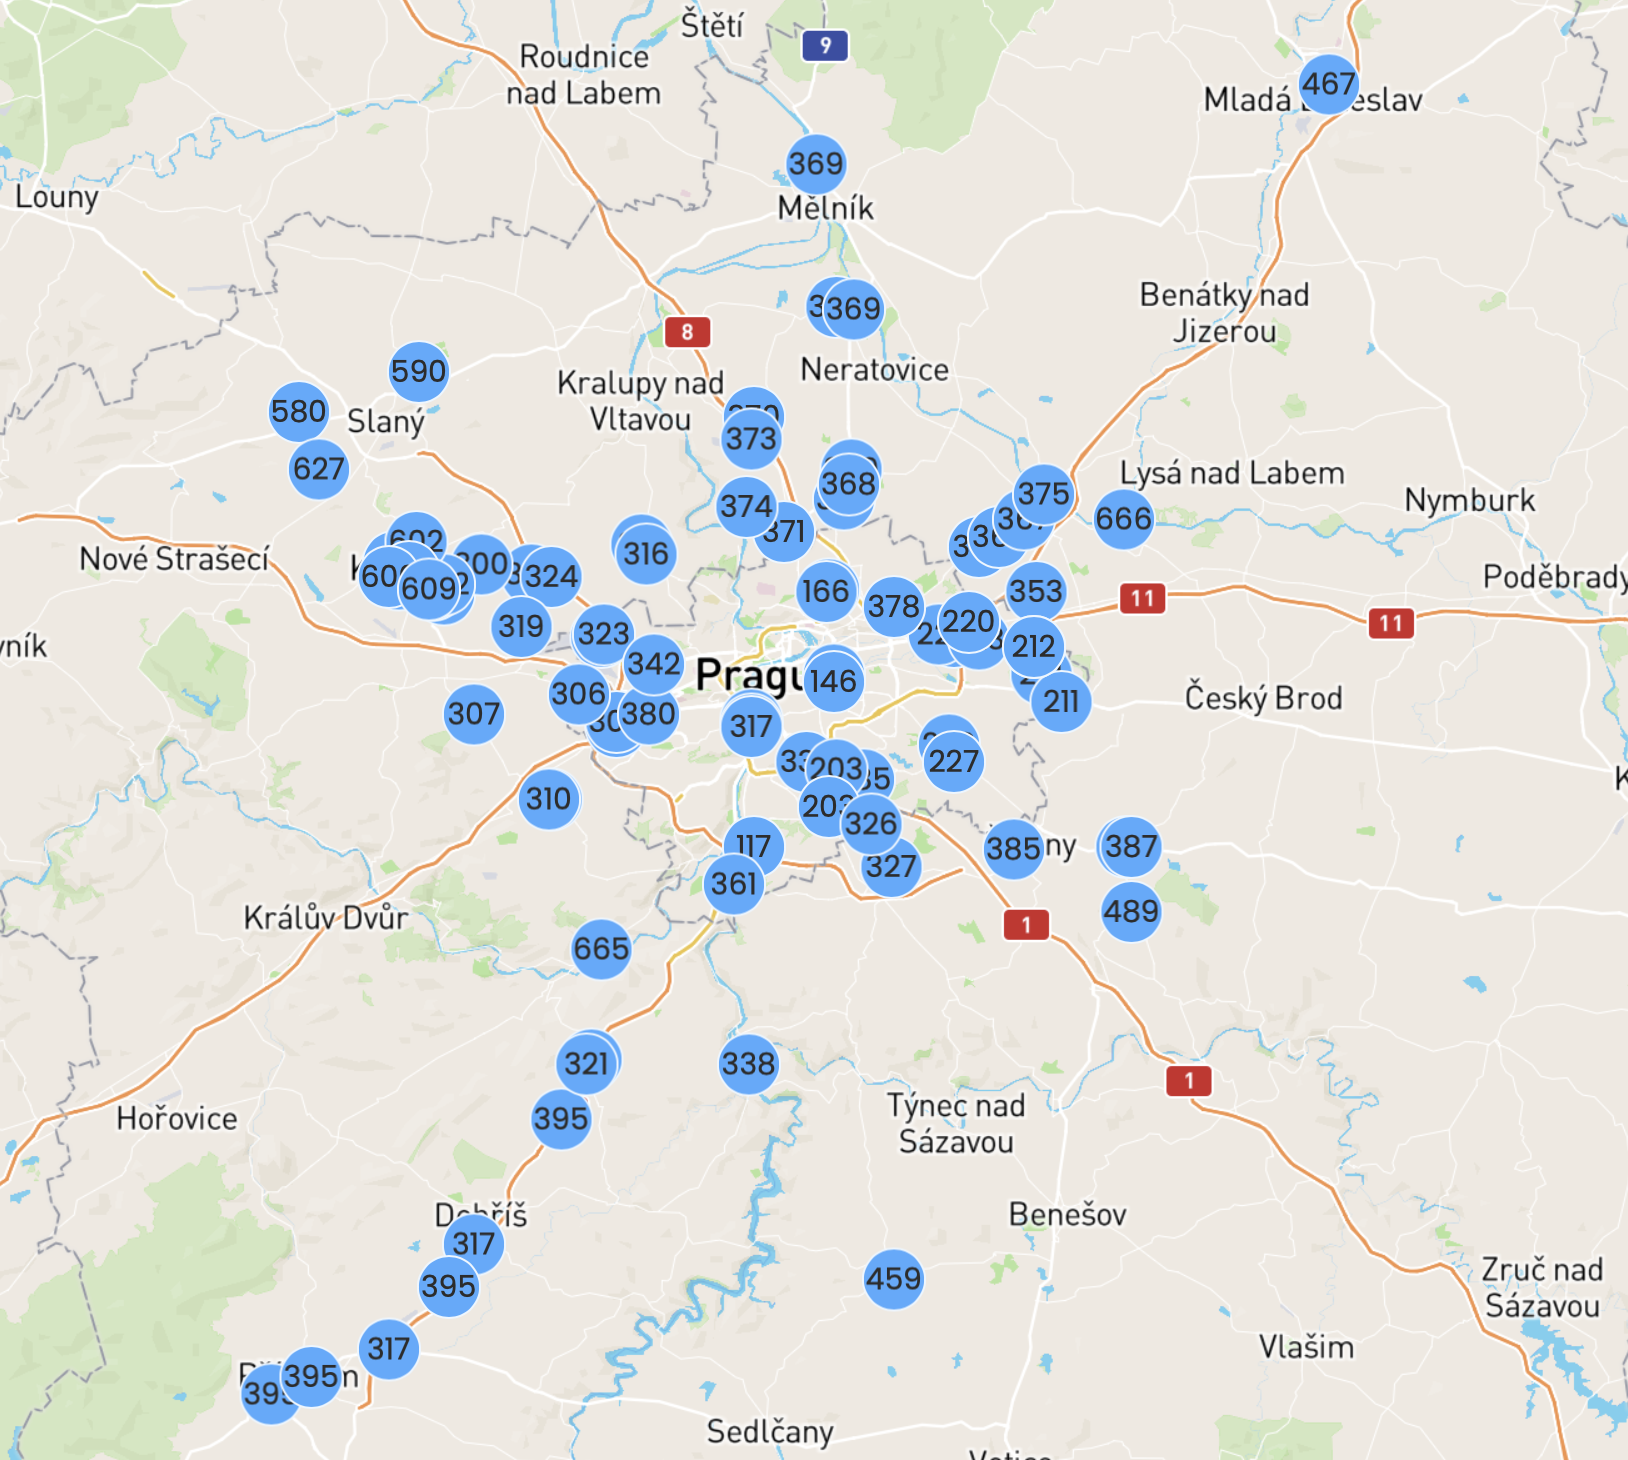
\includegraphics[width=0.7\linewidth]{../img/big_picture.png}
 \caption{Mapa Prahy a~okolí s~polohy vozidel zaznamenány 23.\,2.\,2020}
 \label{fig:big_picture}
\end{figure}


\begin{figure}
   \centering
 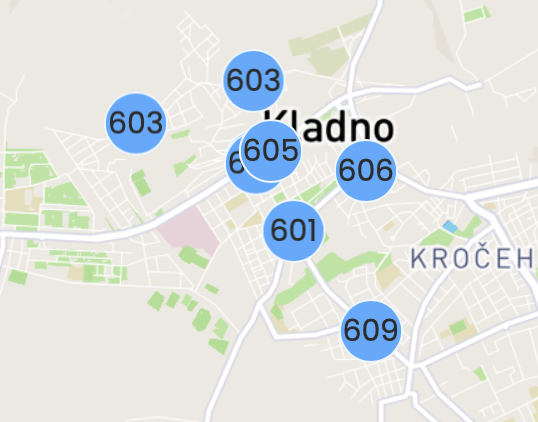
\includegraphics[width=0.3\linewidth]{../img/cluster.png}
 \caption{Shluk vozidel}
 \label{fig:cluster}
\end{figure}


\bigbreak


Dále se v~pořádku zobrazily i~přídavné informace o~vybraném vozidle. Tedy všechny zastávky, kterými spoj projíždí (kterých může být i~několik desítek) a~tabulka s~jízdním řádem. Na obrázku \ref{fig:trip_path} je vidět zobrazení celé trasy spoje. Vybraný spoj je zvýrazněn a~vždy se zobrazí přes všechny ostatní ikony jiných vozidel. Jízdní řád spoje se pak zobrazí v~tabulce zobrazené na obrázku \ref{fig:kladno_aut_322}.


\begin{figure}
   \centering
 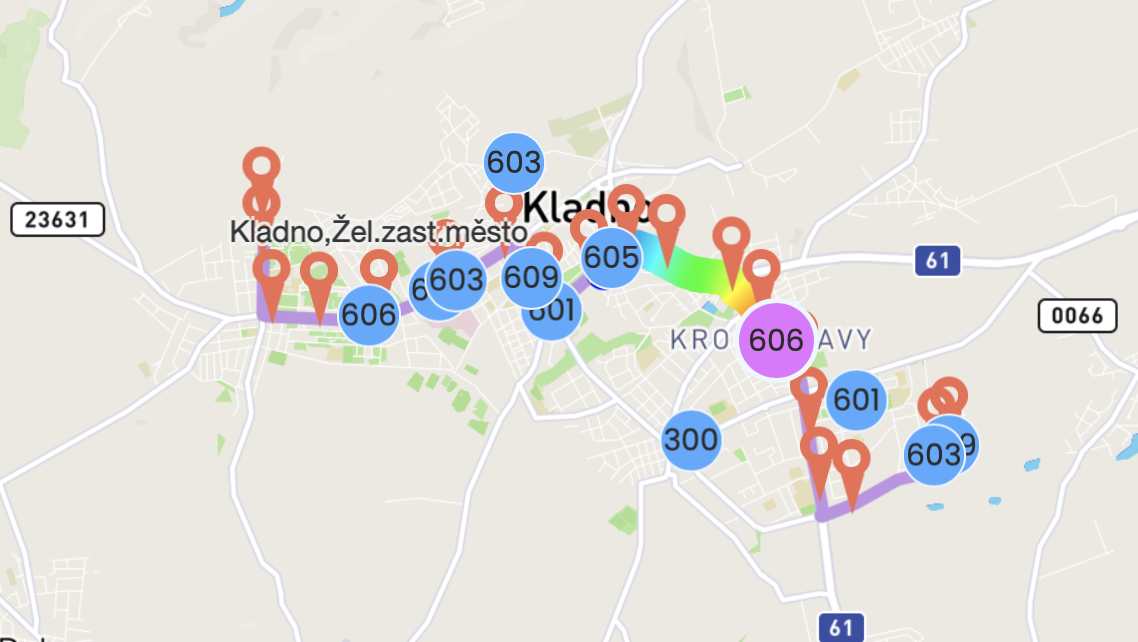
\includegraphics[width=0.7\linewidth]{../img/trip_path.png}
 \caption{Vyznačená trasa jízdy}
 \label{fig:trip_path}
\end{figure}


\begin{figure}
   \centering
 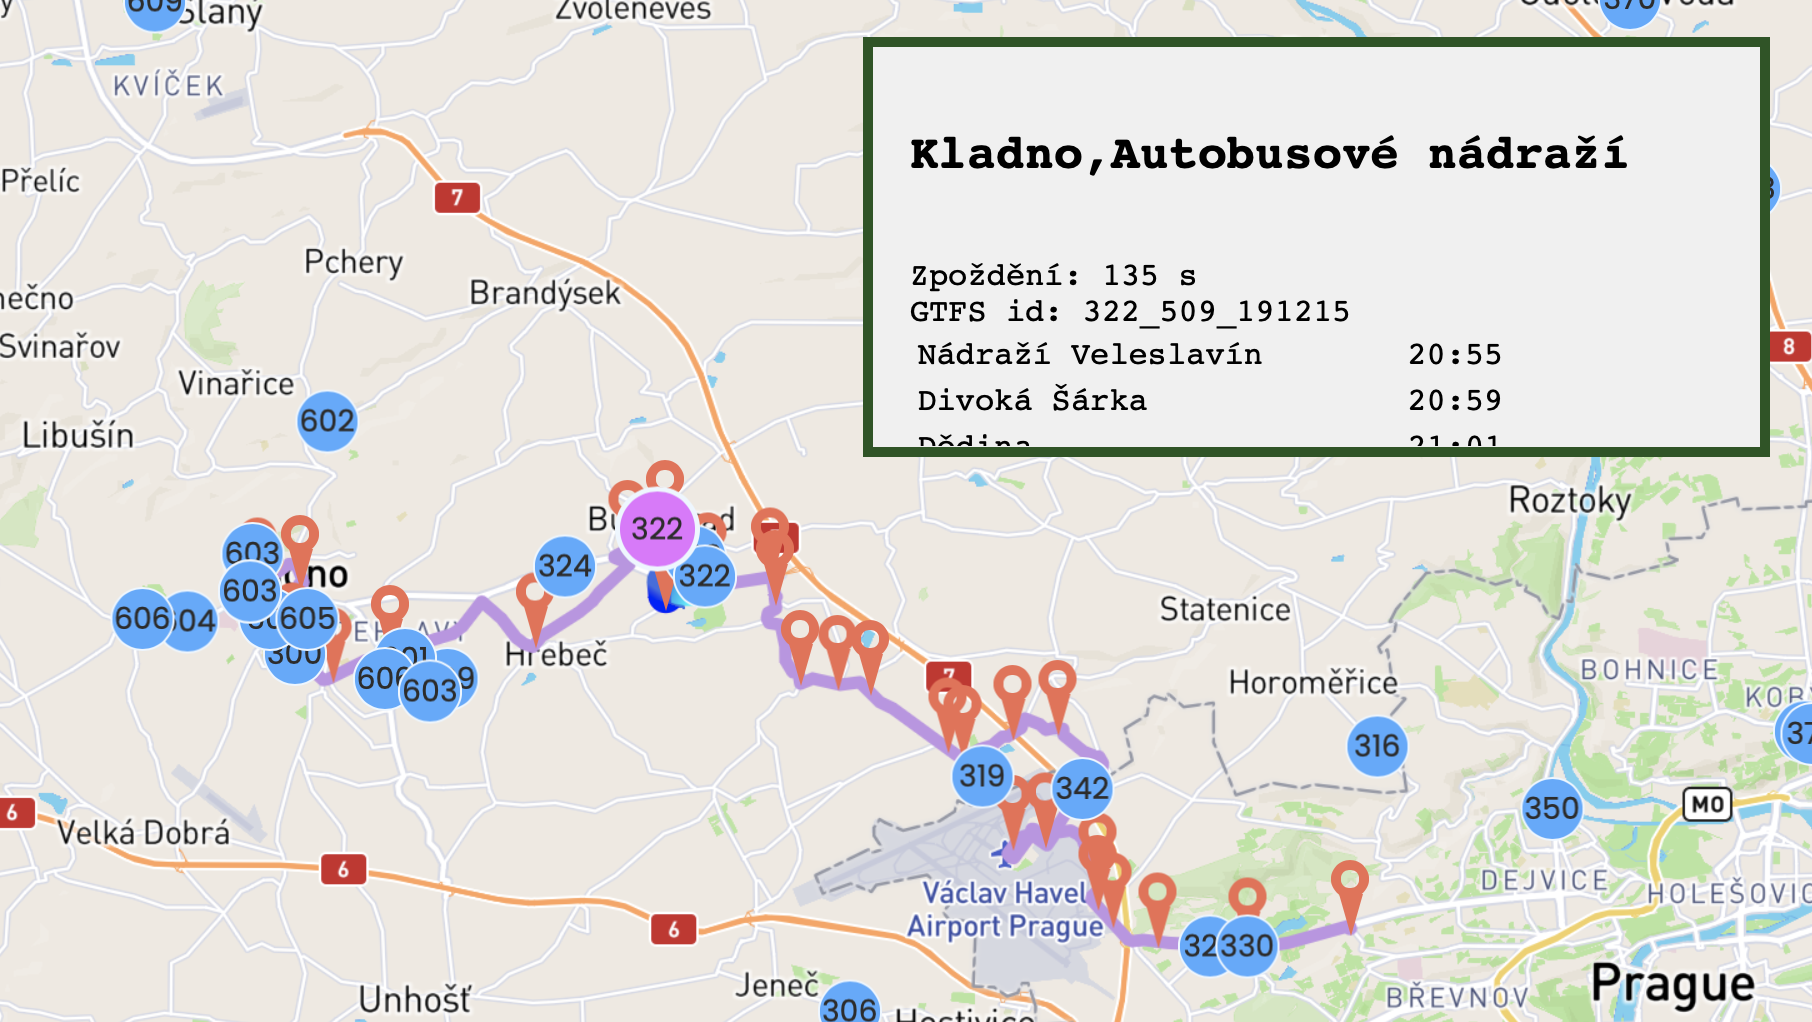
\includegraphics[width=0.7\linewidth]{../img/kladno_aut_322.png}
 \caption{Vyznačená trasa jízdy s~jízdním řádem}
 \label{fig:kladno_aut_322}
\end{figure}


\bigbreak

Pokud byla vybrána zastávka, zobrazila se odjezdová tabule a~všechny spoje, které budou zastávkou projíždět\footnote{V demonstrační aplikaci se zobrazí všechny spoje projíždějící zastávkou, protože časy jízdních řádů neodpovídají simulovaným časům pořízení vzorků poloh vozidel.}. Zobrazení více vozidel současně je ilustrováno na obrázku \ref{fig:more_trips}. Odjezdová tabule je zobrazena na obrázku \ref{fig:stredokluky_table}


\begin{figure}
   \centering
 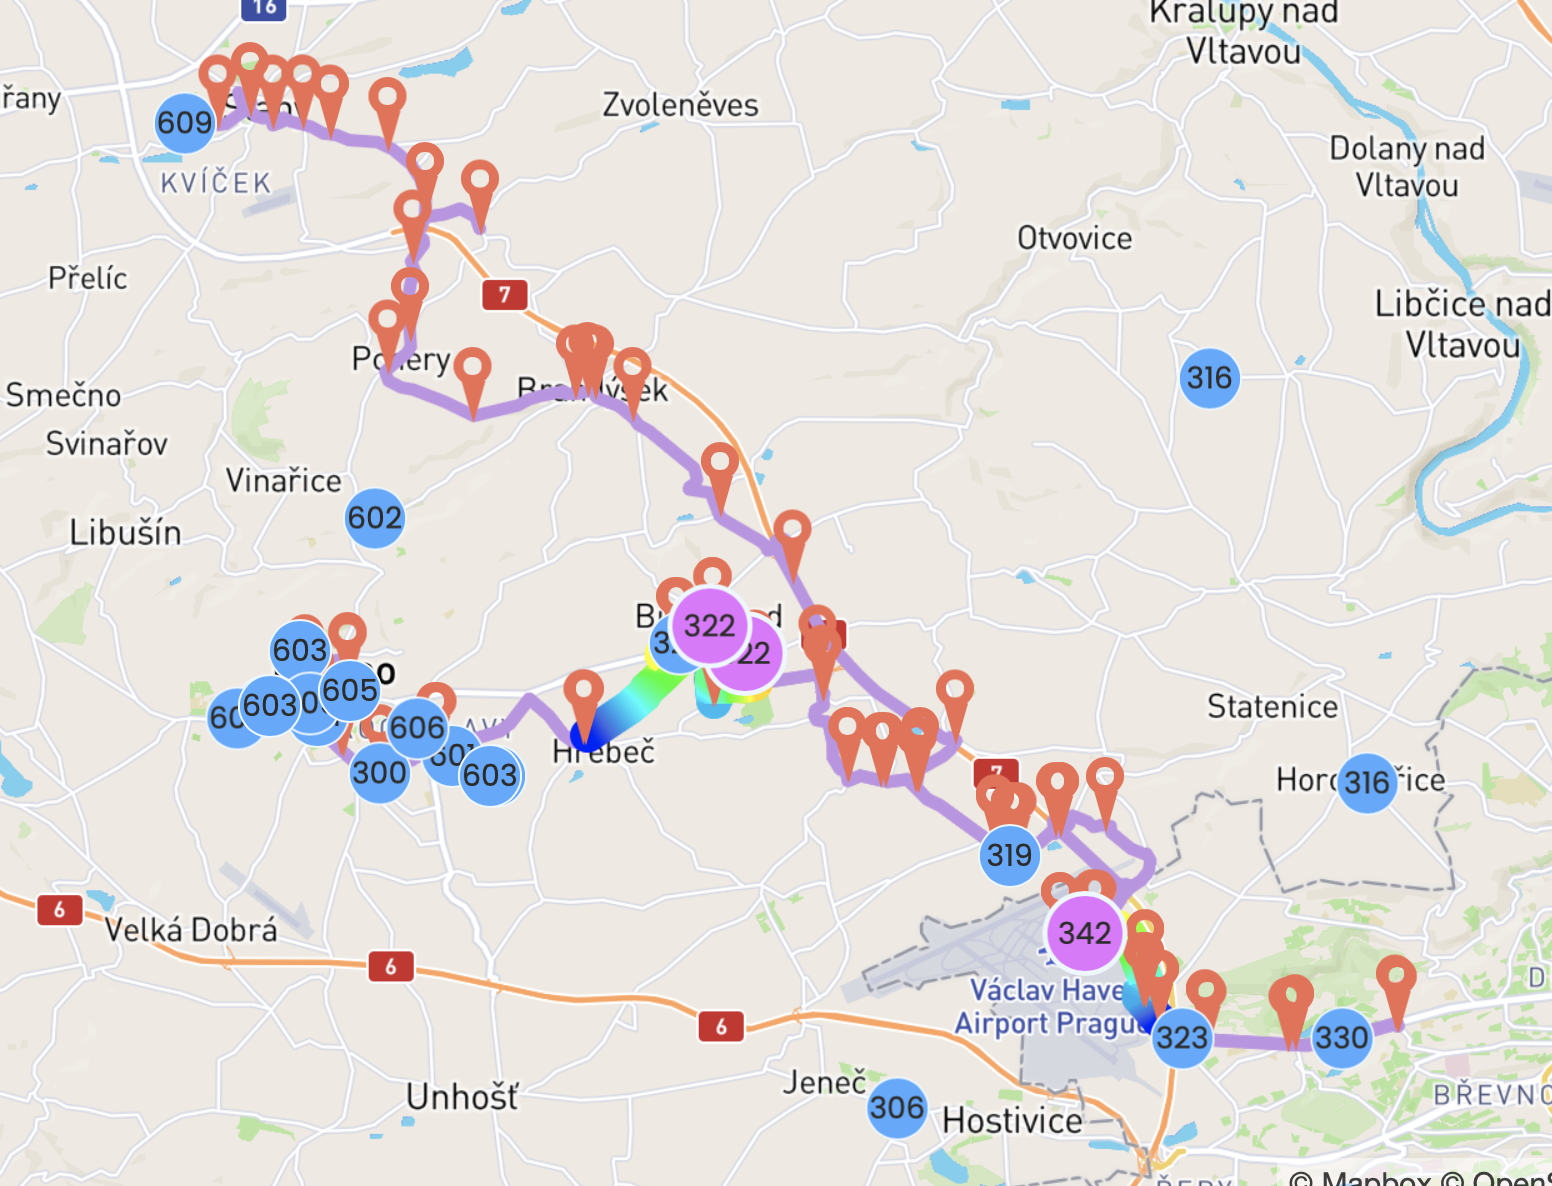
\includegraphics[width=0.7\linewidth]{../img/more_trips.png}
 \caption{Vozidla projíždějící vybranou zastávkou}
 \label{fig:more_trips}
\end{figure}


\begin{figure}
   \centering
 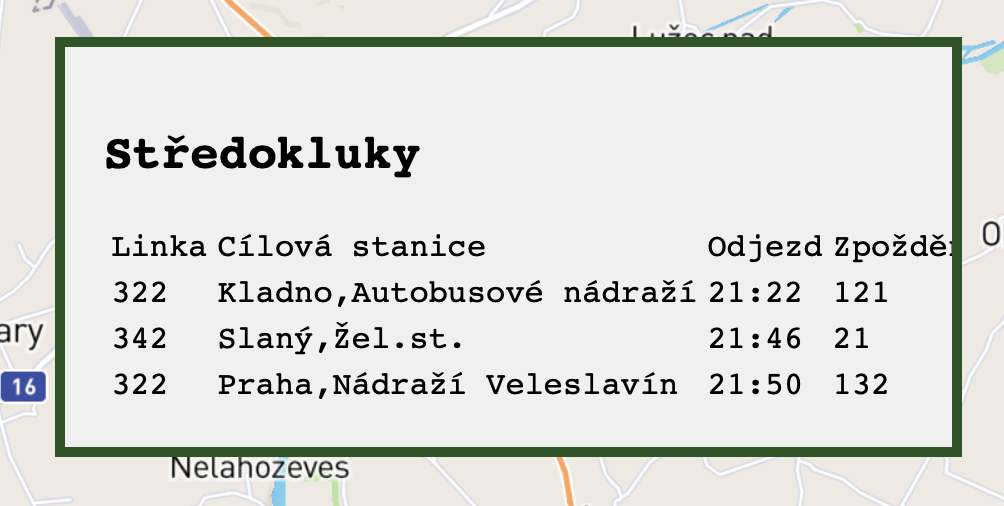
\includegraphics[width=0.4\linewidth]{../img/stredokluky_table.png}
 \caption{Odjezdová tabule}
 \label{fig:stredokluky_table}
\end{figure}


\section{Evaluace výsledků}

\subsection{Konstrukce modelů}

Zde popsaná data vychází z~trénování modelů na datech sbíraných ve dnech 20.\,2.\,2020 -- 23.\,2.\,2020, tedy ze 4~dnů (2~pracovních, 2~víkendových).


\bigbreak

Z 2\,142 dvojic zastávek se alespoň pro jeden typ dne (pracovní, víkendový) vytvořil polynomiální model popisující profil jízdy mezi nimi pro 1\,108 dvojic zastávek. Pro oba typy dnů se polynomiální model vytvořil ve 222 případech. Ve 190 případech se vytvořil model pouze pro pracovní dny, protože mezi danou dvojicí zastávek nejel žádný spoj ve víkendový den.


\bigbreak

Chceme-li zjistit, jak přesně jsou profily jízdy odhadnuty pomocí vytvořených modelů, zaměříme se na \gls{rmse} u~každého modelu. Tato chyba nám říká, o~kolik sekund se v~průměrném případě náš odhad plete od skutečnosti na testovacích datech\footnote{Jedná se o~testovací data, podle kterých se určil nejlepší stupeň polynomu. Kdy vstupní data pro funkci trénování modelu byla rozdělena na trénovací a~testovací. Testovací data, podle kterých posuzujeme vlastnosti nově odhadnutých zpoždění v~kapitole \ref{subsection:odhady_zpozdeni}, jsou zcela jiná množina dat \citep[viz][Strana 365, validation set a~test set]{Ripley96}.}. Pro pracovní dny je průměrná \gls{rmse} necelých 20 sekund. Nejvyšší \gls{rmse} byla zaznamenána 200 sekund. Tak vysoké odchylky jsou, po prozkoumání jednotlivých případů způsobeny chybami ve vstupních datech, které se automaticky odstraňují jen velmi obtížně. Příklad je zobrazen na grafu \ref{fig:chyba_zpozdeni_v_posledni_zastavce}. V~tomto konkrétním případě jsou chybně uvedena zpoždění v~poslední projeté zastávce. Histogram všech \gls{rmse} modelů z~pracovních dnů je zobrazen na grafu \ref{fig:rmse}. Zde je patrné, že nejčastěji je chyba do 30 sekund a~zcela výjimečně překročí 60 sekund. Takto nízké chyby jsou nad očekávání dobré, protože průměrných 20 sekund je pro cestujícího čekající na autobus takřka nepostřehnutelnými.


\begin{figure}
   \centering
 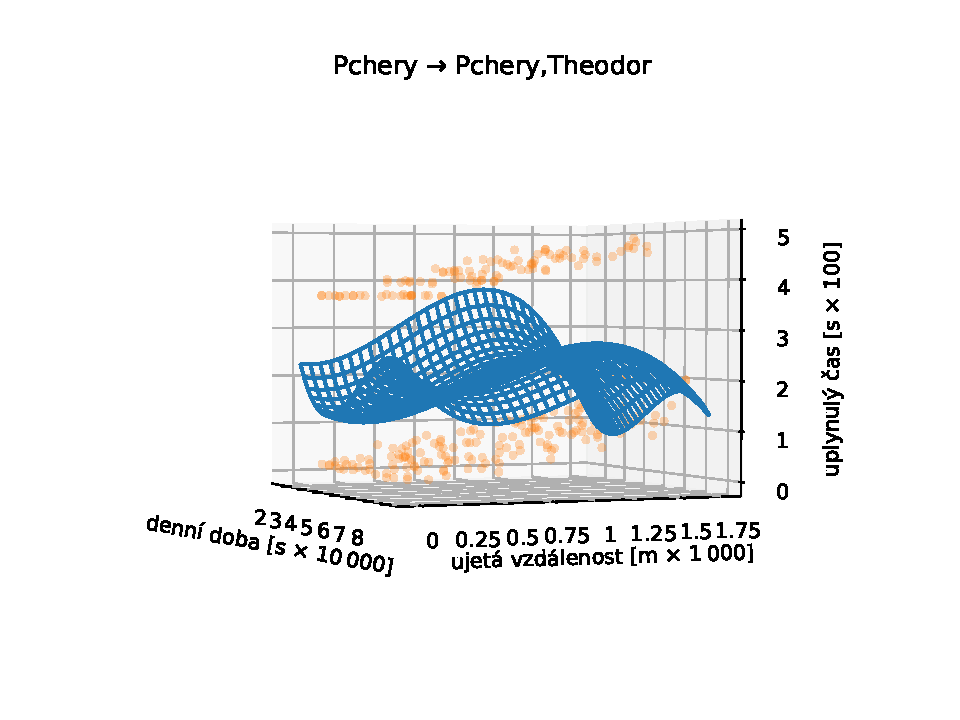
\includegraphics[width=\linewidth]{../img/134_135}
 \caption{Modelování profilu jízdy s~chybnými vstupními daty}
 \label{fig:chyba_zpozdeni_v_posledni_zastavce}
\end{figure}


\begin{figure}
   \centering
 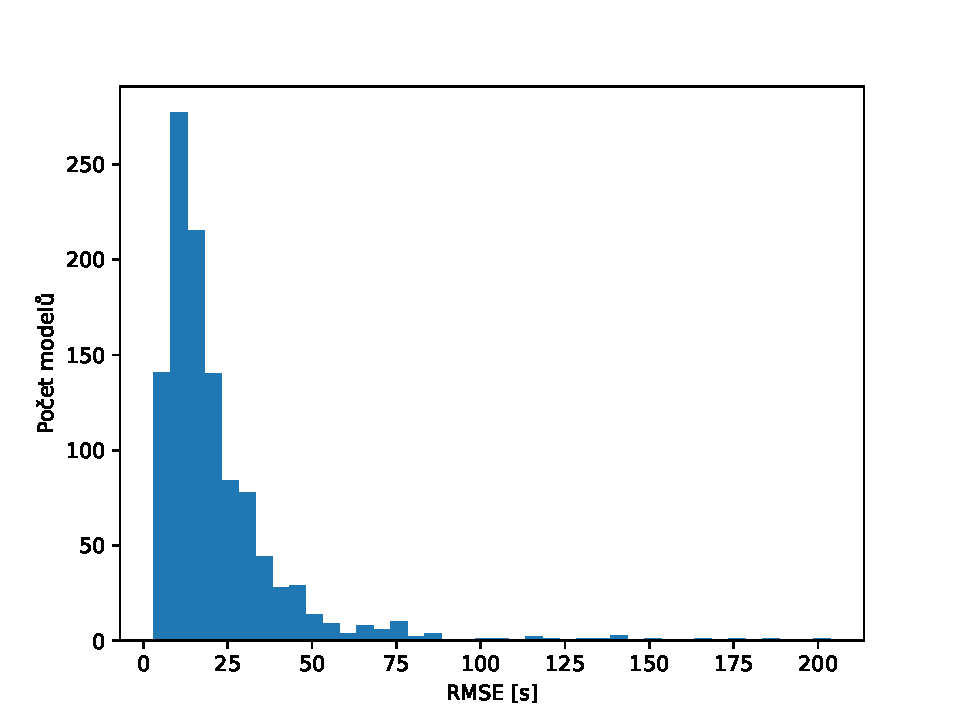
\includegraphics[width=\linewidth]{../img/rmse}
 \caption{Histogram \gls{rmse} všech modelů}
 \label{fig:rmse}
\end{figure}


\bigbreak

Co se týče stupňů polynomiálních regresí, které využíváme při konstrukci modelů, tak nejčastěji se generoval model stupně 3~nebo~4. Což značí, že průběhy tras jsou poměrně tvárné. Modely vyššího stupně se nalezly také, ale spíše značí chybu v~datech, protože se tak snaží vymodelovat různě rozházené vzorky, jako třeba na obrázku \ref{fig:chyba_zpozdeni_v_posledni_zastavce}. Nakonec se nalezlo i~nezanedbatelné množství modelů stupně~2, což také značí tvárnost, ale převážně jen v~jedné ose. Vizualizace modelu druhého řádu je na grafu \ref{fig:second_degree}, třetího řádu na grafu \ref{fig:thrd_degree}


\begin{figure}
   \centering
 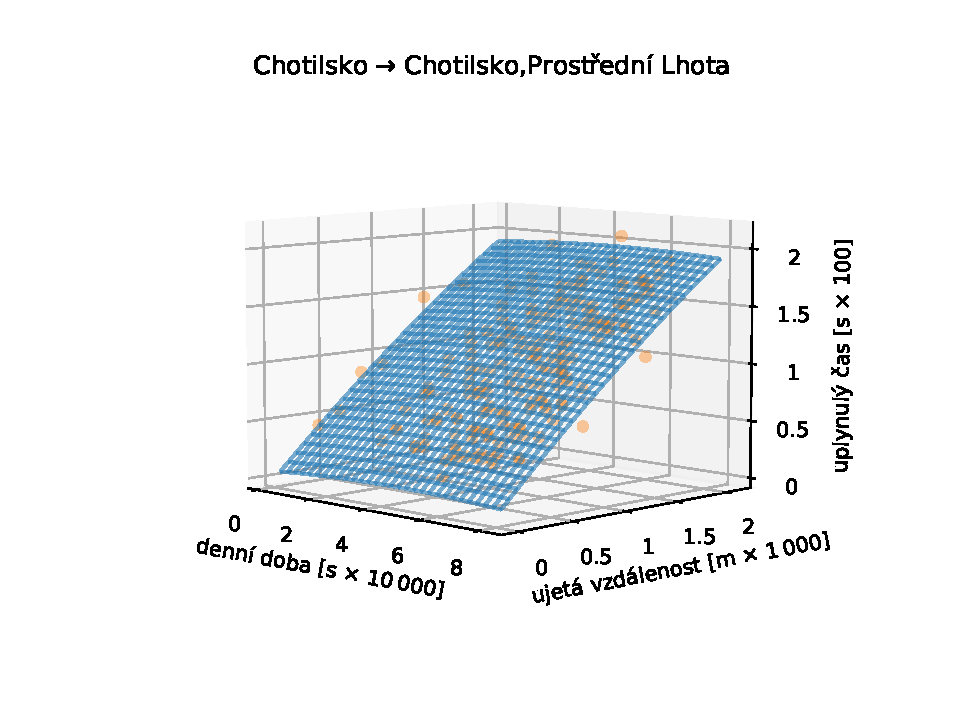
\includegraphics[width=\linewidth]{../img/23_24}
 \caption{Vizualizace modelu druhého stupně}
 \label{fig:second_degree}
\end{figure}

\begin{figure}
   \centering
 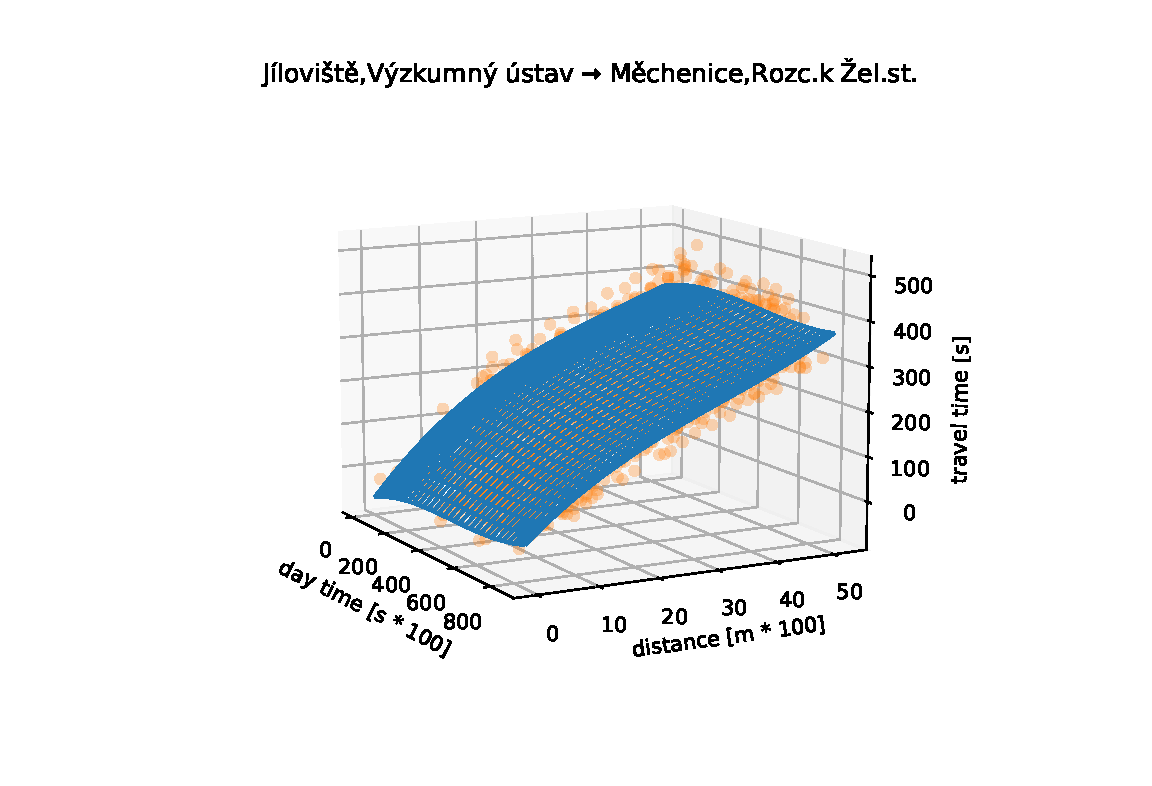
\includegraphics[width=\linewidth]{../img/thrd_degree}
 \caption{Vizualizace modelu třetího stupně}
 \label{fig:thrd_degree}
\end{figure}


\subsection{Odhady zpoždění} \label{subsection:odhady_zpozdeni}

Z toho, jak jsou definovány požadavky řešení v~kapitole \ref{subsubsection:kvalitativni_pozadavky} pro změření kvality výsledků, stačí porovnávat odhad zpoždění lineárního (původního) modelu a~nového polynomiálního modelu. Přičemž odhad je lepší, pokud má sekvence odhadů zpoždění z~celé jízdy mezi dvojicí zastávek menší rozptyl\footnote{Níže budeme pracovat s~odmocninou z~rozptylu, což se formálně nazývá směrodatná odchylka.}.


\bigbreak

Podívejme se tedy na porovnání odhadů zpoždění novými modely profilů jízd se stávajícím řešení pracujícím s~předpokladem, že vozidla jedou celou trasu mezi dvěma zastávkami konstantní rychlostí. Budeme porovnávat data pouze mezi dvojicí zastávek, mezi kterými byl spočítán polynomiální model. V~jiných případech, kdy model spočítán nebyl, se vždy použil lineární model a~není tedy co srovnávat.


\bigbreak

Evaluaci výsledků budeme provádět s~daty sesbíranými 20.\,2.\,2020, které použijeme jako trénovací data a~s daty sesbíranými 21.\,2.\,2020, které použijeme jako testovací data. Toto je standardní postup pro hodnocení úspěšnosti predikcí modelů ve světě strojového učení. Modely nemohou být testovány na stejných datech, jako na kterých byly trénovány, protože kdyby se trénovalo i~testovalo na stejných datech, model by nemusel nic predikovat, ale stačilo by, aby si jen \uv{zapamatoval} hodnotu z~množiny trénovacích dat \citep[viz][Strana 30]{Gareth13}.

\bigbreak

Z dat sesbíraných 20.\,2.\,2020 se vytvořilo 284 modelů popisující průběh trasy.


\bigbreak

Budeme porovnávat zaznamenaná odhadnutá zpoždění mezi odhadem podle lineárního modelu a~polynomiálního modelu. Pro lepší výsledky vyloučíme z~porovnání vzorky poloh vozidel, které byly zaznamenány bezprostředně po vyjetí z~první zastávky nebo před přijetím do druhé zastávky. Takové vzorky poloh vozidel obsahují často chybná data, která negativně ovlivňují výpočet modelů (data jsou vyloučena i~při výpočtu) i~porovnání jejich výsledků. Tyto chyby jsou převážně způsobeny zaokrouhlováním atributu ujeté vzdálenosti ve vzorku dat na celé stovky.

\bigbreak

Ilustrujme si tento problém na příkladu z~reálných dat. V~tabulce \ref{table:9270_samples} jsou zaznamenány vybrané polohy vozidla, které jelo podle jízdního řádu, jehož první dvě zastávky jsou uvedené v~tabulce \ref{table:9270_ride}. Ačkoli je druhá zastávka spoje ve vzdálenosti 4\,840 metrů o~výchozí zastávky, podle vzorku polohy vozidla pořízeném ve vzdálenosti 4\,800 metrů se změnilo zpoždění v~poslední zastávce, což značí, že vozidlo již stojí v~druhé zastávce. Avšak kdybychom brali všechny vzorky dat pořízené před projetím bodu 4\,840 metrů (druhá zastávka), zahrneme tento bod do výpočtu modelu, resp. evaluace výsledků a~negativně nám ovlivní výsledky. Dále vidíme, že po vyjetí ze zastávky má vozidlo konstantní zpoždění v~poslední projeté zastávce, tedy vozidlo opustilo zastávku a~je na trase.

\begin{center}
   \begin{table}[ht]
\centering
\begin{tabular}{|c|c|c|}
\hline
ID spoje & ujetá vzdálenost & zpoždění v~poslední zastávce \\ \hline \hline
336\_89\_181210 & 4400 & 61 \\ \hline
336\_89\_181210 & 4700 & 61 \\ \hline
336\_89\_181210 & 4800 & 84 \\ \hline
336\_89\_181210 & 4900 & 92 \\ \hline
336\_89\_181210 & 5300 & 92 \\ \hline
\end{tabular}
\label{table:9270_samples}
\caption{Záznamy poloh spoje 336\_89\_181210.}
\end{table}
\end{center}


\begin{center}
   \begin{table}[ht]
\centering
\begin{tabular}{|c|c|}
\hline
ID spoje & vzdálenost zastávky na trase \\ \hline \hline
336\_89\_181210 & 0 \\ \hline
336\_89\_181210 & 4840 \\ \hline
\end{tabular}
\label{tab:9270_ride}
\caption{Výtah z~jízdního řádu spoje 336\_89\_181210.}
\end{table}
\end{center}


\bigbreak


Nyní se podívejme už na samotné srovnání rozptylů zpoždění, které jednotlivé modely odhadovaly na trasách mezi danými dvojicemi zastávek. Histogram rozptylů ke dvojicím zastávek podle lineárního modelu je vidět na grafu \ref{fig:rozptyl_old}. Histogram rozptylů zpoždění podle polynomiálního modelu je zobrazen na grafu \ref{fig:rozptyl_new}. Z~porovnání těchto grafů je jasně viditelné, že došlo k~výraznému zmenšení rozptylu. Průměr rozptylů se snížil z~19 sekund na~12.


\begin{figure}
   \centering
 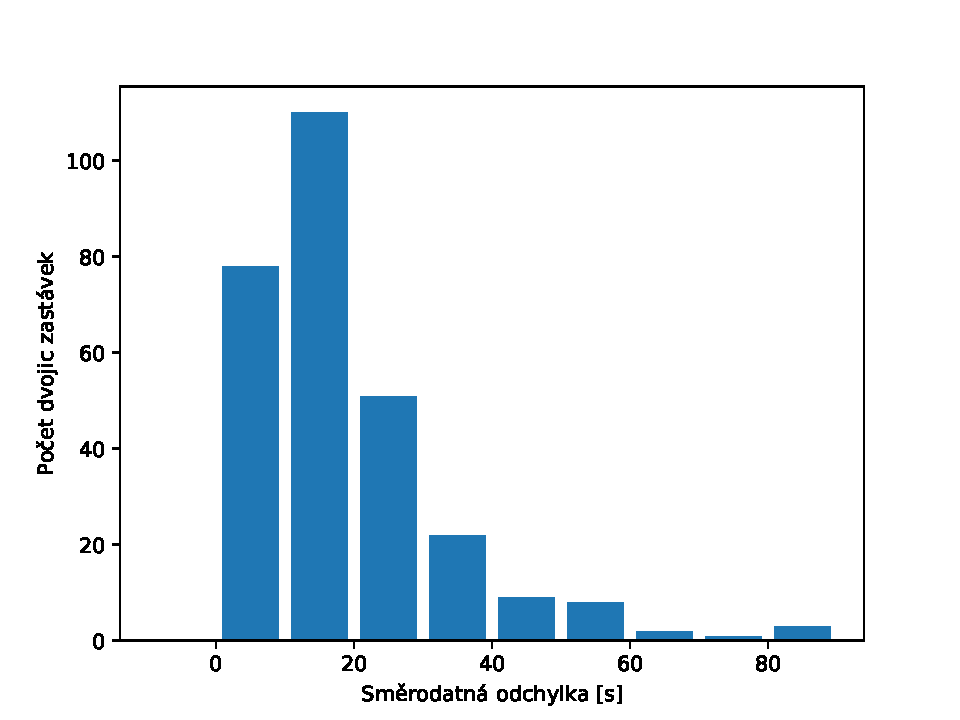
\includegraphics[width=\linewidth]{../img/rozptyl_old}
 \caption{Histogram rozptylu zpoždění podle lineárního modelu, poslední sloupec značí hodnoty 80 a~více}
 \label{fig:rozptyl_old}
\end{figure}


\begin{figure}
   \centering
 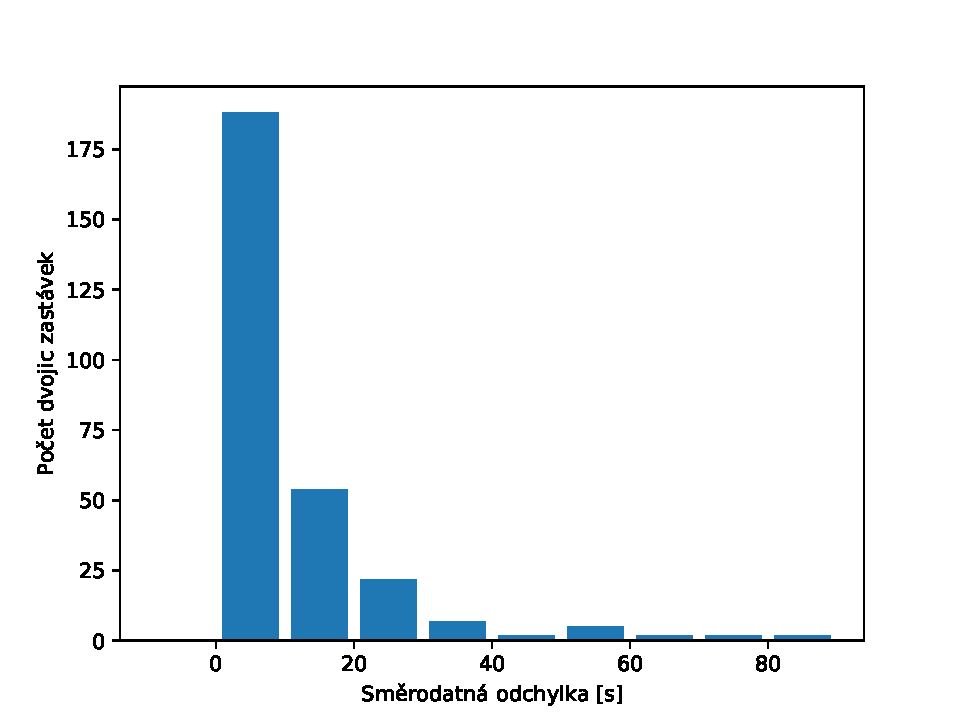
\includegraphics[width=\linewidth]{../img/rozptyl_new}
 \caption{Histogram rozptylu zpoždění podle polynomiálního modelu, poslední sloupec značí hodnoty 80 a~více}
 \label{fig:rozptyl_new}
\end{figure}


\bigbreak

Tyto grafy nám ukazují, že v~průměru došlo ke zlepšení odhadu, ale podívejme se ještě na porovnání rozptylů zpoždění mezi dvojicemi zastávek jednotlivě. Na histogramu \ref{fig:rozptyl_diff} je patrné, že u~největšího počtu dvojic zastávek došlo ke snížení rozptylu o~0 až 10 sekund, nezanedbatelného počtu dvojic o~10 až 20 sekund a~k významnému snížení došlo u~necelých 25 dvojic. Toto pozorování lze vyvodit i~z grafů \ref{fig:rozptyl_old} a~\ref{fig:rozptyl_new}, ze kterých vychází, že k~nejvýznamějšímu poklesu rozptylů došlo z~10--20 sekund na 10--20 sekund.


\begin{figure}
   \centering
 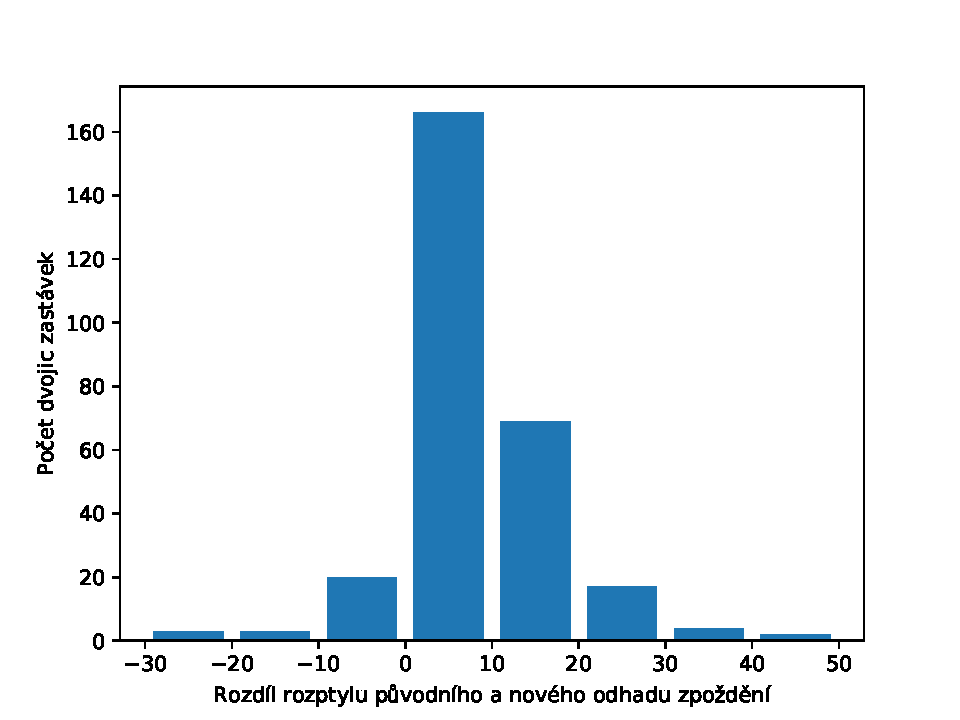
\includegraphics[width=1\linewidth]{../img/rozptyl_diff}
 \caption{Histogram rozdílu rozptylu zpoždění podle lineárního modelu a~polynomiálního modelu}
 \label{fig:rozptyl_diff}
\end{figure}


\subsubsection{Příklad zhoršení odhadu zpoždění}

Dále také na grafu \ref{fig:rozptyl_diff} vidíme, že u~26 dvojic došlo ke zvýšení rozptylu, což je v~této práci nežádoucí. Stalo se tak, ale pouze v~necelých 10 procentech případů a~z toho ve většině nedošlo k~výraznému zhoršení. Avšak v~jednotkách případů došlo k~výraznému zhoršení i~o několik desítek sekund. Rozeberme si tedy jeden příklad výrazného zhoršení, a~proč k~němu došlo.


\bigbreak

Na grafu \ref{fig:chyba} je vizualizován vygenerovaný model pro dvojici zastávek, kde došlo k~největšímu zhoršení oproti odhadu zpoždění lineárním modelem. Na první pohled se zdá, že takto model vypadá správně. Při bližším ohledání ale zjistíme, že dokonalá vlna vznikla z~chybných vstupních dat. Konkrétně si povšimneme, že vzorky se seskupily do dvou clusterů, první ve vzdálenosti 0 až 3\,000 metrů od vyjetí a~druhý dále.


\begin{figure}
   \centering
 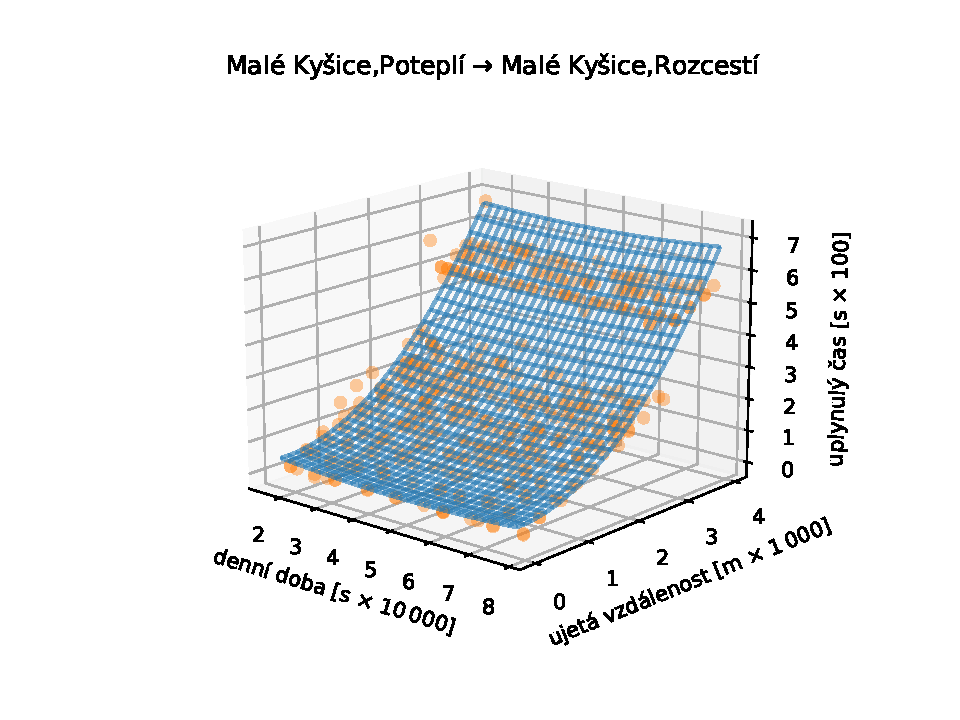
\includegraphics[width=1\linewidth]{../img/808_809}
 \caption{Zhoršení odhadu zpoždění vlivem špatných vstupních dat}
 \label{fig:chyba}
\end{figure}


Chybná vstupní data, ze kterých vypočítaný model vychází, uvedeme ještě v~tabulce \ref{table:825_samples} a~část jízdního řádu dotčeného spoje v~tabulce \ref{tab:825_ride}. V~první tabulce si můžeme povšimnout, že zhruba ve dvou třetinách jízdy mezi zastávkami došlo ke změně zpoždění v~poslední zastávce. Což je z~našeho pohledu nevysvětlitelné. Tento skok ve zpoždění o~více než 220 sekund je u~všech jízd projíždějících mezi touto dvojicí zastávek.


\begin{center}
   \begin{table}[ht]
\centering
\begin{tabular}{|c|c|c|}
\hline
ID spoje & ujetá vzdálenost & zpoždění v~poslední zastávce \\ \hline \hline
630\_177\_200210 & 6700 & 167 \\ \hline
630\_177\_200210 & 7400 & 167 \\ \hline
630\_177\_200210 & 7600 & 167 \\ \hline
630\_177\_200210 & 7900 & 167 \\ \hline
630\_177\_200210 & 8300 & -62 \\ \hline
630\_177\_200210 & 8600 & -62 \\ \hline
630\_177\_200210 & 9100 & -62 \\ \hline
\end{tabular}
\label{table:825_samples}
\caption{Záznamy poloh spoje 630\_177\_200210.}
\end{table}
\end{center}


\begin{center}
   \begin{table}[ht]
\centering
\begin{tabular}{|c|c|}
\hline
ID spoje & vzdálenost zastávky na trase \\ \hline \hline
630\_177\_200210 & 5225 \\ \hline
630\_177\_200210 & 9187 \\ \hline
\end{tabular}
\label{tab:825_ride}
\caption{Výtah z~jízdního řádu spoje 630\_177\_200210.}
\end{table}
\end{center}


\bigbreak

Avšak tento skok by se měl projevit i~u odhadu zpoždění lineárním modelem. Jak je tedy možné, že u~lineárního modelu vyšel rozptyl velmi malý a~u polynomiálního modelu v~řádu vysokých desítek? K~pochopení nám napomůže podívat se na záznamy tohoto spoje v~den 21.\,2.\,2020, tedy na záznamy, které slouží pro evaluaci úspěšnosti. V~tento den se totiž pořídily pouze 3~záznamy ve vzdálenosti 2\,km od sebe. Tedy lineární model předpověděl všem téměř stejná zpoždění, ale polynomiální model vlivem natrénování se na špatných datech, odhadoval zpoždění zcela mimo realitu.


\bigbreak

Z tohoto se dá usuzovat, že v~případech, kde se rozptyl zpoždění výrazně zhoršil, jsou na vině závady ve vstupních datech nebo nám schází informace o~procesu určování zpoždění v~poslední projeté zastávce. Např.: i~autobusy mohou projíždět návěstidly, kde se po průjezdu hodnota zpoždění upraví, avšak z~jízdních řádů takovou informaci nezjistíme.


\subsubsection{Příklad zlepšení odhadu zpoždění}

Na druhou stranu v~našem modelovém případě profilu jízdy mezi zastávkami K~Letišti a~Zličín pro spoj 324\_593\_200106 došlo k~výraznému zlepšení, a~tedy snížení rozptylu z~60 sekund na 12. Kompletní porovnání záznamu vývoje zpoždění na trase je možné pozorovat na grafu \ref{fig:compare_534_421}.


\begin{figure}
   \centering
 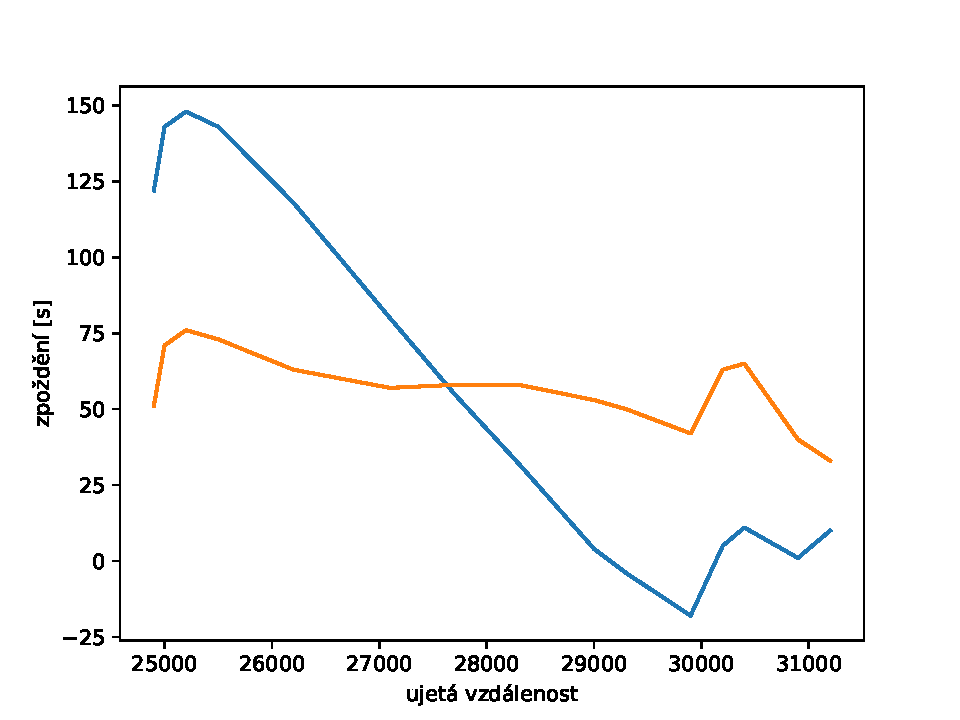
\includegraphics[width=1\linewidth]{../img/compare_534_421}
 \caption{Porovnání průběhu odhadnutých zpoždění lineárním modelem (modrá) a~polynomiálním modelem (oranžová) mezi zastávkami K~Letišti a~Zličín}
 \label{fig:compare_534_421}
\end{figure}


\section{Statistiky} \label{section:stats}

Ze sesbíraných dat je možné odvozovat i~různé statistiky o~spojích nebo o~zpoždění jízd. Uveďme si tedy některé z~nich.

\bigbreak

Všechny uvedené grafy a~statistiky se zakládají na datech ze dne 20.\,2.\,2020.


\bigbreak

Na prvním grafu \ref{fig:trips_len} je znázorněn histogram celkových délek jízd všech spojů. Přičemž průměrná délka jízdy spoje byla 18 kilometrů.

\begin{figure}
   \centering
 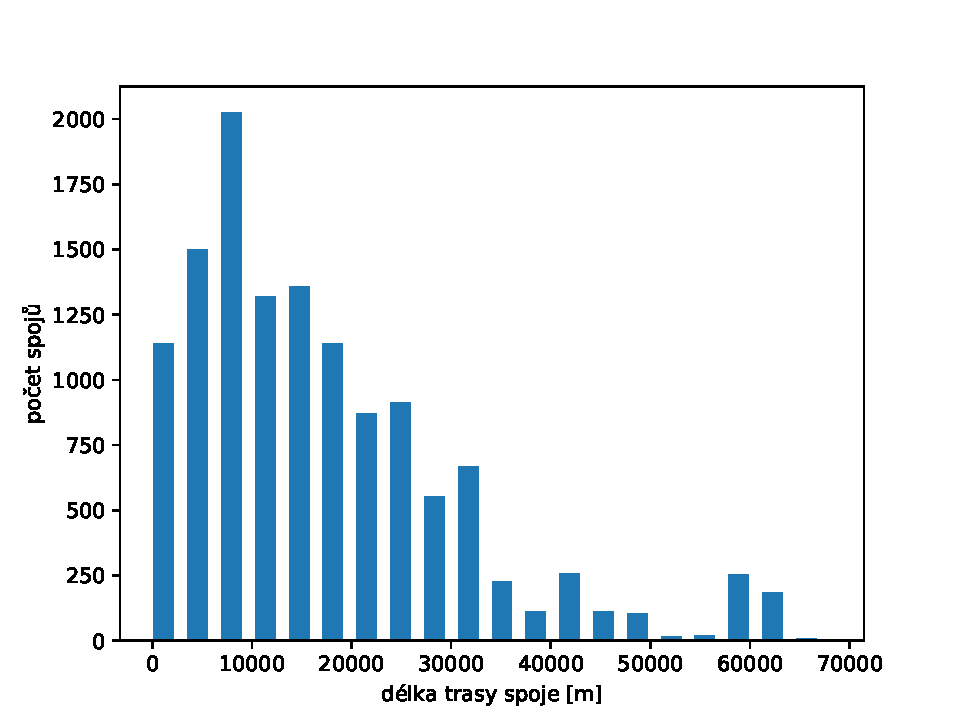
\includegraphics[width=1\linewidth]{../img/trips_len}
 \caption{Histogram délek tras spojů.}
 \label{fig:trips_len}
\end{figure}


\bigbreak

Dále si uveďme, počet zastávek, které jeden spoj obsluhuje. Samotný histogram se podobá předešlému histogramu \ref{fig:trips_len} zachycující délky jízd, proto jen v~číslech. Průměrný počet zastávek jednoho spoje je~17. Rekordní počty zastávek jsou přitom 2~a~48. Celkem 2~zastávky obsluhuje 192 spojů, ale většina z~nich jsou přívozy P1 a~P2, které se také dostaly do naší databáze a~18 spojů autobusů také obsluhuje pouze 2~zastávky\footnote{Vysvětleme proč 2 přívozy tvoří většinu spojů oproti 18 spojům pozemní dopravy. Jedna linka je obsluhována několika spoji (spoj se váže na konkrétní jízdní řád), ale linka je daná sekvencí zastávek. Protože přívozy jezdí poměrně často, jsou popsány velkým množstvím spojů. Ale dotčené autobusové linky jezdí méně často, proto jim přísluší menší počet spojů.}. Naopak maximální počet zastávek na trase má pouze 8~spojů, které náleží jedné lince číslo 369.


\bigbreak


Na grafu \ref{fig:trips_total_delay} je zobrazeno zpoždění všech jízd v~jejich konečné stanici\footnote{Pokud zpoždění v~konečné stanici nebylo dostupné ve vstupních datech, bylo použito zpoždění v~předposlední stanici.} a~celková délka jejich trasy. Intuitivně by se mohlo říci, že s~rostoucí délkou trasy bude zpoždění narůstat. Ale jak vychází z~grafu průměrné zpoždění v~závislosti na délce trasy je takřka konstantní. Průměrné zpoždění činilo 114 sekund a~rozptyl byl 179 sekund. Z~toho vychází, že většina jízd dojela se zpožděním, byť v~řádu jednotek minut, ale zároveň tím dochází k~minimalizaci počtu jízd, které přijedou v~předstihu. V~konečné zastávce nás sice toto může potěšit, ale musíme si uvědomit, že celkové předjetí se akumuluje po celou dobu jízdy a~na zastávkách před konečnou stanicí by tedy vozidlo muselo čekat.


\begin{figure}
   \centering
 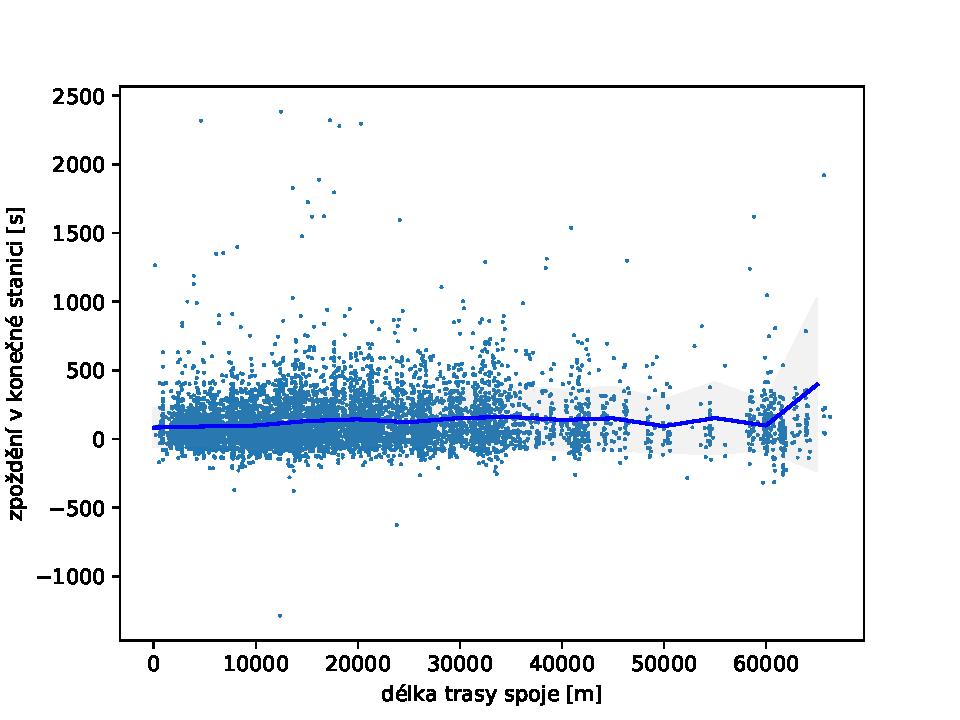
\includegraphics[width=1\linewidth]{../img/trips_total_delay}
 \caption{Zpoždění v~poslední zastávce jízdy vůči délce celé trasy jízdy, Průměr vyznačen modře a~rozptyl šedě}
 \label{fig:trips_total_delay}
\end{figure}
